\begin{blocksection}
\question Draw the environment diagram that results from running the code.

\begin{lstlisting}
def bar(f, x):
    if x == 1:
        return f(x)
    else:
        return f(x) + bar(f, x - 1)

f = 4
bar(lambda x: x + f, 2)
\end{lstlisting}

\begin{solution}[0.3in]
Output: 3 \newline
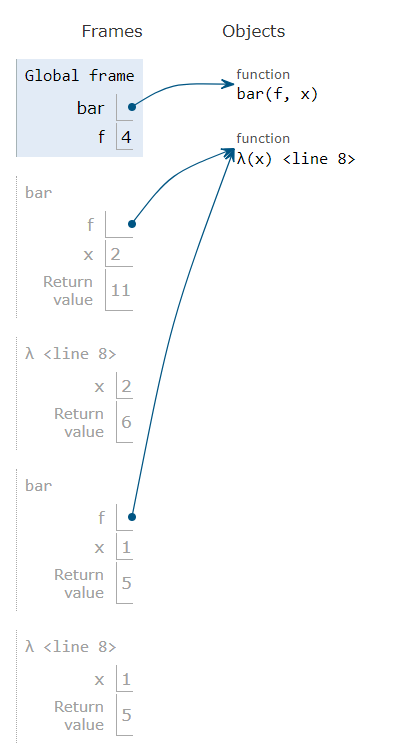
\includegraphics[scale=0.5]{foobar1_new.png}
\newline
\url{https://goo.gl/kR2n9M}
\end{solution}
\end{blocksection}
